\part{Computer memory}
\frame{\partpage}

\begin{frame}{What does this circuit do?}
	\centering
	\begin{circuitikz} \draw[color=\circuitcolour]
		(0,0) node[nand port] (gateA) {}
		(0,-2) node[nand port] (gateB) {}
		(gateA.out) -- ($ (gateA.out) + (0, -0.5) $) -- ($ (gateB.in 1) + (0, 0.5) $) -- (gateB.in 1) {}
		(gateB.out) -- ($ (gateB.out) + (0, 0.5) $) -- ($ (gateA.in 2) + (0, -0.5) $) -- (gateA.in 2) {}
		(gateA.out) -- ($ (gateA.out) + (0.5, 0) $) node[anchor=west] {$Q$}
		(gateB.out) -- ($ (gateB.out) + (0.5, 0) $) node[anchor=west] {$\overline{Q}$}
		(gateA.in 1) -- ($ (gateA.in 1) + (-0.5, 0) $) node[anchor=east] {$S$}
		(gateB.in 2) -- ($ (gateB.in 2) + (-0.5, 0) $) node[anchor=east] {$R$}
		;
	\end{circuitikz}
	\begin{itemize}
		\pause\item This is called a \textbf{NAND latch}
		\pause\item It ``remembers'' a single boolean value
		\pause\item Put a few billion of these together
			(along with some control circuitry)
			and you've got \textbf{memory}!
	\end{itemize}
\end{frame}

\begin{frame}{Memory}
	\pause
	\begin{center}
		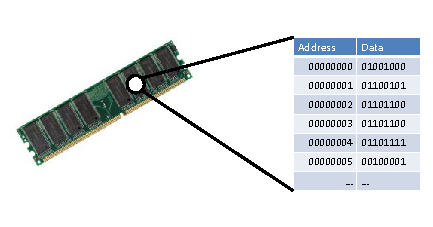
\includegraphics[width=0.8\textwidth]{memory}
	\end{center}
	\begin{itemize}
		\item Memory works like a set of \textbf{boxes}
		\pause\item Each box has a number, its \textbf{address}
		\pause\item Each box contains a \textbf{byte} (8 bits)
	\end{itemize}
\end{frame}

\begin{frame}{Data representation} 
	\begin{itemize}
		\pause\item Memory stores \textbf{sequences of numbers}
		\pause\item Therefore, any data stored by a computer must be represented as a sequence of numbers
			\begin{itemize}
				\pause\item Text: sequence of ASCII (or Unicode etc) character codes
				\pause\item Image: sequence of pixel colour values
				\pause\item 3D model: sequence of vertex coordinates
				\pause\item Audio: sequence of displacements
				\pause\item Executable: sequence of machine code operations
			\end{itemize}
	\end{itemize}
\end{frame}
